\documentclass{article}
\usepackage[margin=0.7in]{geometry}
\usepackage{amsmath}
\usepackage{amssymb}
\usepackage{graphicx}


\begin{document}

\section{Introduction}

I, with the help of Devojyoti, wrote these codes to investigate the effect of linear and non-linear polarisation calibration schemes, under various conditions. In particular, I have tested the cases, where the instrumental leakage is low and high. Under each possibility, I have also investigated the effect when the source has high and low polarisation fractions. For the linear calibration scheme, I have used CASA. For the non-linear calibration scheme, I have used quartical as well as a code I wrote. While the codes were developed by me, I have discussed the details of the procedure with Devojyoti and we are in complete agreement about the results and the methodology. So, this is really a joint effort and should be treated as such. In the spirit of reproducibility, we thought that it is better to upload all codes used in this work on Github, along with a detailed description of the steps which is needed to run this code as well as the understanding we get from it.


\section{Simulating visibilities}

Let us denote the jones matrix corresponding to antenna $i$, which describes the leakage matrix, as 

\begin{equation}
J^{leakage}_i=
\begin{pmatrix}
1 & d_{xi}e^{i\phi_{xi}} \\
d_{yi}e^{i\phi_{yi}} & 1
\end{pmatrix}
\end{equation}

Both $d_{xi}$s and $d_{yi}$s are chosen from randomly from a uniform distribution. For the low leakage case, the uniform distribution corresponding to $(0.01,0.07)$. For the high leakage case, the limits are $(0.15,0.25)$. $\phi_{xi}$ and $\phi_{yi}$ are drawn from a gaussian distribution with mean of $50^\circ$ and sigma of $10^\circ$. We also use a crosshand phase ($\theta$) to be $50^\circ$. Thus the combined Jones matrix for each antenna $i$ is given by

\begin{equation}
J_i=\begin{pmatrix}
1 & d_{xi}e^{i\phi_{xi}} \\
d_{yi}e^{i\phi_{yi}} & 1
\end{pmatrix} 
\begin{pmatrix}
\cos \theta & \sin \theta\\
-\sin \theta & \cos \theta
\end{pmatrix}
\end{equation}

The visibilities for baseline corresponding to the antenna pair $(p,q)$ for a source with Stokes parameters $(I,Q,U,V)$ are predicted as

\begin{equation}
\begin{pmatrix}
V_{pq,RR} & V_{pq,RL}\\
V_{pq,LR} & V_{pq,LL}
\end{pmatrix}=0.5 F J_p 
\begin{pmatrix}
I+V & Q+iU\\
Q-iU & I-V
\end{pmatrix}J_q^\dagger, \quad \text{$F$ is the Fourier Transform operator}
\end{equation}

We simulate the visibilities for 5 point sources, the properties of which are given in Table \ref{tab:source_props}

\begin{table}[!htbp]
\centering
\begin{tabular}{c|c|c|c|c}
Source name & I & Q & U & V  \\\hline
$S_1$ & 10 & 0 & 0 & 0\\
$S_2$ & 50 & 1 & 5  & 0\\
$S_3$ & 50 & 5 & 1 & 0\\
$S_4$ & 50 & 4 & 15 & 0\\
$S_5$ & 50 & 15 & -5 & 0
\end{tabular}
\caption{Model properties of the sources simulated}
\label{tab:source_props}
\end{table}

The goal of this experiment is to investigate how each of the algorithms fare in recovering these input source properties after calibration.

The simulated MS can be generated in the following way.

\begin{enumerate}
\item If low leakage case, first run \textit{simulate\_leakages.py} in the low\_leakages folder. Similarly,for different cases, we run the codes with same name, but located in its own corresponding folder.
\item Create a folder called CASA, quartical and self\_crosshand inside the folder. If you have the github code, then the folders already exist.
\item Copy a GMRT MS (band2\/band3\/band4, just to ensure that the polarization is stated as RR\/LL in the MS header), such that it has only 1 channel and 1 time. Name the MS es should be as follows: 'CASA/unpolarized\_source\_I10.ms', 'CASA/polarized\_source\_I50\_Q1\_U5\_V0.ms',  'CASA/polarized\_source\_I50\_Q5\_U1\_V0.ms',
 'CASA/polarized\_source\_I50\_Q4\_U15\_V0.ms',    'CASA/polarized\_source\_I50\_Q15\_neg\_U5\_V0.ms'
 \item Next run simulate\_vis\_polarized\_all.py after changing the file names appropriately.
\end{enumerate}

\section{Low leakage}

\subsection{Linear analysis}

Linear analysis under each test scenario can be performed by running the script named polcalibrate\_CASA.py located inside the CASA folder in each test case.

In the linear regime, we can solve for relative leakages in the circular basis.  Hence, for accurate comparison, we have used a reference antenna to solve for the leakages. When comparing with the input leakages, we have appropriately computed the relative leakage of each antenna with respect to the reference antenna. In Figure \ref{fig:linear_CASA_leak_comparison}, we show the comparison between the relative input and solved leakages. The script named compare\_leakage\_model.py inside the CASA folder is run to produce this figure. It is evident that the relative leakages solved matches exacty with the relative input leakages. Next, we have solved for the crosshand phase using $S_1$. Then we apply all the solved parameters to all sources. In Figure \ref{fig:compare_input_output_source_params}, we compare the model and recovered source linear polarization properties for sources $S_2\cdots S_5$. We observe a very tiny deviation in the recovered polarisation angle compared to the model. The script, compare\_model\_corrected.py, is run after using the appropriate figure names to generate this figure.

\begin{figure}
\centering
\includegraphics[scale=0.5]{/home/barnali/Downloads/surajit/leakage_test/low_leakage_case/CASA/casa_solved_leakage_comparison.png}
\caption{XX}
\label{fig:linear_CASA_leak_comparison}
\end{figure} 

\begin{figure}
\centering
\includegraphics[trim={2cm 0 2cm 0},clip,scale=0.7]{/home/barnali/Downloads/surajit/leakage_test/low_leakage_case/CASA/compare_calibrated_values.pdf}
\caption{XX}
\label{fig:compare_input_output_source_params}
\end{figure}

\subsection{Nonlinear analysis}

Nonlinear analysis, using quartucal, under each test scenario can be performed by running the bash script named analyse\_quartical.sh located inside the quartical folder in each test case. 

Comparing the determined leakages using quartical with the input has another issue. We note here that quartical solves a matrix of the following form when use the {\it{leakage}} form.

$$
\begin{pmatrix}
1 & d_{xi}e^{i\phi_{xi}} \\
d_{yi}e^{i\phi_{yi}} & 1 
\end{pmatrix}
$$

 As mentioned in Kansabanik et al. 2024, the optimizing equation, which uses the Frobenius norm, is degenerate with respect to a unitary matrix. This implies that the leakage matrix determined using quartical has an unknown unitary matrix\footnote{the effect of this multiplication during calibration is discussed in detail later in the high leakage case}. multiplied with it, which makes it not comparable directly with the input leakages. To do proper comparison, we take the following approach. The approach has been mentioned in Kansabanik et al. 2024. Here, we mention the procedure for completeness purposes.

Let us assume that the leakage matrix determined by quartical for the reference antenna and a general antenna $i$ are denoted by $J_{ref}$ and $J_i$ respectively. The normalized Jones matrix for each antenna is then given by 
\begin{align}
J_{ref}=&H_{ref}U_{ref}\\
J_{norm,i}=&J_i J_{ref}^{-1}H_{ref}
\end{align}

The input $J^{leakage}_i$ is also normalised in the same manner, using the same reference antenna. Then they are compared, and the comparison is shown in Figure \ref{fig:nonlinear_quartical_leak_comparison}. This figure can be generated by running the script, compare\_quartical\_model\_leak1.py, located inside the quartical folder. In Figure \ref{fig:compare_input_output_source_params_nonlinear} we show the comparison between the input and recovered source parameters. The agreement is slightly better than what we find with CASA, but not sufficiently to say that CASA has performed poorly.

\begin{figure}
\centering
\includegraphics[scale=0.5]{/home/barnali/Downloads/surajit/leakage_test/low_leakage_case/quartical/quartical_solved_leakage_comparison.png}
\caption{XX}
\label{fig:nonlinear_quartical_leak_comparison}
\end{figure}

\begin{figure}
\centering
\includegraphics[trim={2cm 0 2cm 0},clip,scale=0.7]{/home/barnali/Downloads/surajit/leakage_test/low_leakage_case/quartical/compare_calibrated_values.pdf}
\caption{XX}
\label{fig:compare_input_output_source_params_nonlinear}
\end{figure}

\section{High leakage}

The most general case is implemented in a folder named high\_leakage\_case\_general. 

\subsection{Linear analysis}

The CASA analysis is exactly similar and the codes which are run are also named same. In Figure \ref{fig:linear_CASA_leak_comparison_high_leak_high_leak_general}, we show the comparison between the relative input and solved leakages. We find that the solved leakages match exactly with the input leakage, after appropriate normalisation. This is not surprising, considering that the cross-hand visibilities are exactly same for unpolarized source both in the linear and non-linear regime. In Figure \ref{fig:compare_input_output_source_params}, we compare the model and recovered source polarization properties for sources $S_2\cdots S_5$. We observe large deviations in the recovered polarisation properties compared to the model. In fact, the Stokes I is different for the recovered source, in comparison to the input source model. We have verified that the I and V after calibration is same as that in the data, after corruption by the antenna Jones matrices. This demonstrates that CASA does not apply leakage corrections and crosshand corrections to the co-polar visibilities.

\begin{figure}
\centering
\includegraphics[scale=0.5]{/home/barnali/Downloads/surajit/leakage_test/high_leakage_case_general/CASA/casa_solved_leakage_comparison.png}
\caption{XX}
\label{fig:linear_CASA_leak_comparison_high_leak_general}
\end{figure} 

\begin{figure}
\centering
\includegraphics[trim={2cm 0 2cm 0},clip,scale=0.7]{/home/barnali/Downloads/surajit/leakage_test/high_leakage_case_general/CASA/compare_calibrated_values.pdf}
\includegraphics[scale=0.6]{/home/barnali/Downloads/surajit/leakage_test/high_leakage_case_general/CASA/recovered_polarisation_properties.png}
\caption{XX}
\label{fig:compare_input_output_source_params_high_leak_general}
\end{figure}



\subsection{Nonlinear analysis: Quartical}

Here, we also follow the strategy described in the linear case. We solve for the leakage matrices, and then use them to determine the crosshand phase matrix. All of the Jones matrices are determined using quartical. The analysis code is again named  analyse\_quartical.sh, located in a folder named quartical\_leakage. The comparison between the leakages after appropriate normalization is shown in Figure \ref{fig:nonlinear_quartical_leak_comparison_high_leak_general}. This figure can be generated by running the script, compare\_quartical\_model\_leak1.py, located inside the quartical folder. In Figure \ref{fig:compare_input_output_source_params_quartical_high_leak_general} we show the comparison between the input and recovered source parameters. The agreement is slightly better than what we find with CASA, in the sense that Stokes I is well matched now. However, Stokes V is roughly of the same order as that determined in the CASA calibration. The question is hence, why even when we are using Quartical, which is a non-linear solver, we can not recovering the input parameters. 

\begin{figure}
\centering
\includegraphics[scale=0.5]{/home/barnali/Downloads/surajit/leakage_test/high_leakage_case_general/quartical_leakage/quartical_solved_leakage_comparison.png}
\caption{XX}
\label{fig:nonlinear_quartical_leak_comparison_high_leak_general}
\end{figure} 

\begin{figure}
\centering
\includegraphics[trim={2cm 0 2cm 0},clip,scale=0.7]{/home/barnali/Downloads/surajit/leakage_test/high_leakage_case_general/quartical_leakage/compare_calibrated_values.pdf}
\includegraphics[scale=0.6]{/home/barnali/Downloads/surajit/leakage_test/high_leakage_case_general/quartical_leakage/recovered_polarisation_properties.png}
\caption{XX}
\label{fig:compare_input_output_source_params_quartical_high_leak_general}
\end{figure}

The answer to this question is quite non-trivial, and has to do the "unitary matrix" degeneracy we mentioned earlier. Remember that we had created a Jones matrix $J^{leakage}_i$ for each antenna. We thought that this matrix will only cause mixing between the Stokes pairs $(I,Q)$, $(I,U)$ and $(I,V)$. However, as we show below, this is not correct.

The $J^{leakage}_{i}$ of each antenna can be written as
\begin{align}
J^{leakage}_i=& J^{leakage}_i \left ( J^{leakage}_{ref} \right )^{-1} H_{ref}U_{ref}\\
J^{leakage}_{ref}=& H_{ref}U_{ref}
\end{align}

$H_{ref},U_{ref}$ are Hermitian and unitary matrices respectively. This suggests that $J^{lekaage}_i$ of each antenna $i$ has a common unitary matrix multiplied with it, and the unitary matrix multiplied depends on the jones matrix of the reference antenna. This unitary matrix is will cause rotation of the Stokes vector in the $Q,U, V$  space, even in absence of any crosshand phase term. Hence, solving for just the crosshand phase will not correct for the entire polrotation term. The reason why Stokes I was ok, was because, the non-linear calibration procedure, has uniuqely determined the polconversion matrix and hence Stokes I is ok when we use Quartical. The solution to this issue is to solve for the full general polrotation matrix. This is done in the next subsection. However, we use the antenna leakages determined using Quartical. We first completely remove the effect of the unitary matrix of the reference antenna and store those in a file. The file is named quartical\_ant\_leaks.txt and can be generated by running get\_quartical\_leak.py . The created txt file is copied from the quartical folder to the folder named self\_crosshand.


\subsection{Nonlinear analysis: Determining the full polrotation matrix} \label{sec:full_porot}

For solving the full polrotation matrix, we need to use at least 2 polarised sources. For this purpose, we use $S_2$ and $S_3$. The code to solve the 3 angles is named solve\_crosshand\_phase.py . The phases are applied to the data using the script named generate\_corrected\_vis.py .  by running the script, compare\_quartical\_model\_leak1.py, located inside the quartical folder. In Figure \ref{fig:compare_input_output_source_params_self_crosshand_high_leak_general} we show the comparison between the input and recovered source parameters. It is evident that all Stokes parameters have been recovered with a much better accuracy. However, in spite of this, we find that Stokes V is still non-zero. This we think is due to numerical errors and convergence parameters chosen in Quartical and our solver used for determining the polrotation matrix.

\begin{figure}
\centering
\includegraphics[trim={2cm 0 2cm 0},clip,scale=0.7]{/home/barnali/Downloads/surajit/leakage_test/high_leakage_case_general/self_crosshand_leakage/compare_calibrated_values.pdf}
\includegraphics[scale=0.6]{/home/barnali/Downloads/surajit/leakage_test/high_leakage_case_general/self_crosshand_leakage/recovered_polarisation_properties.png}
\caption{XX}
\label{fig:compare_input_output_source_params_self_crosshand_high_leak_general}
\end{figure}

\subsection{Does determing the diagonal gains help}

In this section, we try to understand, if it is possible to solve the Stokes V issue, if we were general observers, who had no understanding of how the data was generated. Observers typically does not assume that the diagonal gain is 0. This implies that for quartical, we shal solve for a general matrix using $S_1$. We also run a gaincal before polcal with $S_1$. For the purpose of this, scripts with similar names are present in folders named CASA\_gaincal and quartical In both cases, we find that the estimated amplitude and phase gains are very similar. We show the determined antenna gain terms in Figure \ref{fig:quartical_ant_gains}. The amplitude gains deviation from 1 are about 1--2\%. The phase deviations are also of same order. We otain similar numbers when we use CASA gaincal task as well. We repeat the analysis by applying these parameters, and we find that while CASA results have not changed appreciably, for the non-linear case, Stokes V has improved significantly. In Figure \ref{fig:compare_linear_nonlinear_terms_with_diagonal}, we show the recovered polarization properties from CASA analysis, and the procedure we mentioned in Section \ref{sec:full_porot}. We find that while the non-linear analysis has now recovered all Stokes parameters with an accuracy better than $1\%$, there are quite large errors in the CASA analysis. Observers can solve the spurious Stokes V issue, by running CASA gaincal for each of the calibrator, and then assuming that the gains are varying with time. The determined gain terms are in reality a function of the source polarization properties and the antenna leakages and hence interpolation schemes based on time-variability will not work. 
 
\begin{figure}
\centering
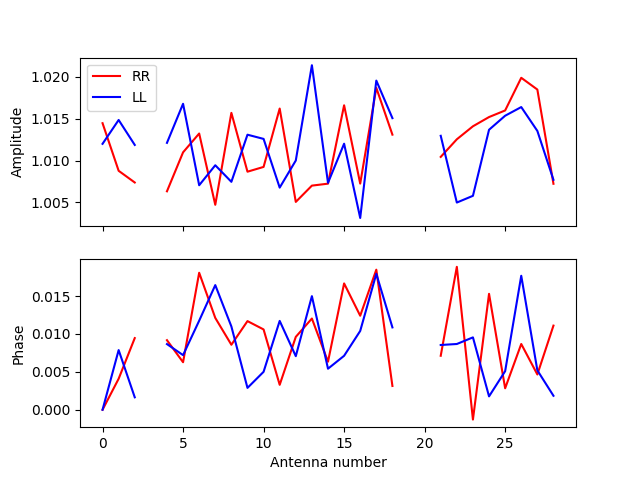
\includegraphics[scale=0.7]{/home/barnali/Downloads/surajit/leakage_test/high_leakage_case_general/quartical/antenna_diagonal_gains.png}
\caption{XX}
\label{fig:quartical_ant_gains}
\end{figure}


\begin{figure}
\centering
\includegraphics[scale=0.5]{/home/barnali/Downloads/surajit/leakage_test/high_leakage_case_general/CASA_gaincal/recovered_polarisation_properties.png}
\includegraphics[scale=0.5]{/home/barnali/Downloads/surajit/leakage_test/high_leakage_case_general/self_crosshand/recovered_polarisation_properties.png}
\caption{XX}
\label{fig:compare_linear_nonlinear_terms_with_diagonal}
\end{figure}


\end{document}